\begin{comment}

According to Luria, purposeful movement is the output of multilevel planning process. It presumes certain goal to be accomplished. 

- The first stage is the general planning, this level answers the question why and how some action should be performed. 

- On the second level, concrete motion patterns are generated on the basis of general plan. These motion patterns are referred as motion melodies. Motion melodies are the sequences of the motions, ordered in time, which should allow accomplishment of the goal. 

- On the third level ”orders” are generated to the direction of the spinal cord. On this level, melody of the motions is implemented. 

The present work is targeted towards detecting disorders on the second and third levels.  Digital Luria’s alternating series test are selected for this purpose.

- The first Luria’s alternating series test: tracing the series requires one to follow the periodic pattern. Tested individual asked to follow periodic pattern, for example sinusoidal line see ”Fig 5” or the line consisting of the strait segments ”Fig 4” (here and after referred as PL - line), with the pen. 

- The second Luria’s alternating test: coping the series requires one to copy periodic pattern. Pattern is drawn on top of the paper and tested individual is asked to draw the same on the bottom of the paper see ”Fig 2 and 3”. 

- The third test: continuing the series, requires one to continue periodic pattern (PL line). Few segments of the pattern are drawn on the paper and tested individual is asked to continue the pattern see ”Fig 1”. 

In a non digitalized case, the neurologist or psychiatrist does assessment visually. If all the tests are problematic for the tested individual then the disorder is most likely on the third level where motion melody is outputted to the spine. Some of the Luria’s tests are quite simple and do not require to generate complicated motion melodies. If the problem appears only during the third (more complicated test), and either do not appear at all or less severe for a simpler tests, then most likely disorder is on the second level where motion melodies are generated.

\end{comment}


\section{Luria's Tests Background}

Human motions, during handwriting and drawing --- are complex multilevel procedures according to Luria's research studies \cite{luria1995higher}. Each complex motion require several phases:

\begin{easylist}[itemize]

& \textit{Motion Planning Phase} --- consists of following sub-phases:
&& \textit{General Planning} --- during initial phase, approximate idea, reason, general representation of the movement are generated in human cortex, along with reason behind the movement and the general representation of how the movement should be executed.

&& \textit{Motion Pattern Creation} --- second phase involves detailed motion pattern generation according to general plan from previous phase. Motion pattern can also be described as series of actions ordered in time.

& \textit{Motion Execution Phase} 
&& \textit{Motion Pattern Implementation} --- series of actions are being implemented during third phase, when pattern is transformed into series of signals to spinal cord.

\end{easylist}

Luria's alternating series tests --- is a proven technique to expose disorders on every phase of motion execution and planning during handwriting process. Test series is represented by combination of certain task types and multiple periodic patterns. 

\subsection{Task types}

Luria alternating series tests are being executed on tablet with stylus. General idea of every test --- to collect handwriting data from tested subject using certain kinds of tasks, listed as follows: 

\begin{easylist}

& \textit{Trace Task} --- implies  tested individual to trace the drawing pattern with stylus exactly above displayed pattern reference image. Simplest task of the series and requires only motion execution phase without complex planning. 

& \textit{Copy Task} --- implies tested individual to reproduce displayed reference pattern with a stylus. Usually reference pattern is displayed on the upper part of screen area. Tested individual is being asked to draw equivalent pattern on a free area of a tablet display. Task requires both motion execution and  planning. May cause difficulties even for healthy subjects, since reference drawing is shown aside, therefore possible borders of the pattern are not obvious.

& \textit{Continue Task} --- implies tested individual to continue and fully complete whole drawing pattern from few visible segments. Most difficult task, both motion execution and complex planning processes are required. May cause difficulties for healthy subjects, since reference drawing is not fully shown, possible borders of required pattern are not obvious.

% - The first Luria’s alternating series test: tracing the series requires one to follow the periodic pattern. Tested individual asked to follow periodic pattern, for example sinusoidal line see ”Fig 5” or the line consisting of the strait segments ”Fig 4” (here and after referred as PL - line), with the pen. 

% - The second Luria’s alternating test: coping the series requires one to copy periodic pattern. Pattern is drawn on top of the paper and tested individual is asked to draw the same on the bottom of the paper see ”Fig 2 and 3”. 

% - The third test: continuing the series, requires one to continue periodic pattern (PL line). Few segments of the pattern are drawn on the paper and tested individual is asked to continue the pattern see ”Fig 1”. 

\end{easylist}

\subsection{Pattern Types}

Possible subset of repetitive drawing \textit{patterns}: \textit{sinus} pattern, \textit{'P'} pattern and \textit{'PL'} pattern. Reasoning behind such naming, is because pattern silhouettes remind Greek letters \textit{Pi} ($\Pi$) and \textit{Lambda} ($\Lambda$). All patterns are presented on following Figure \ref{luria}.

\begin{figure}[htb]
  \centering
    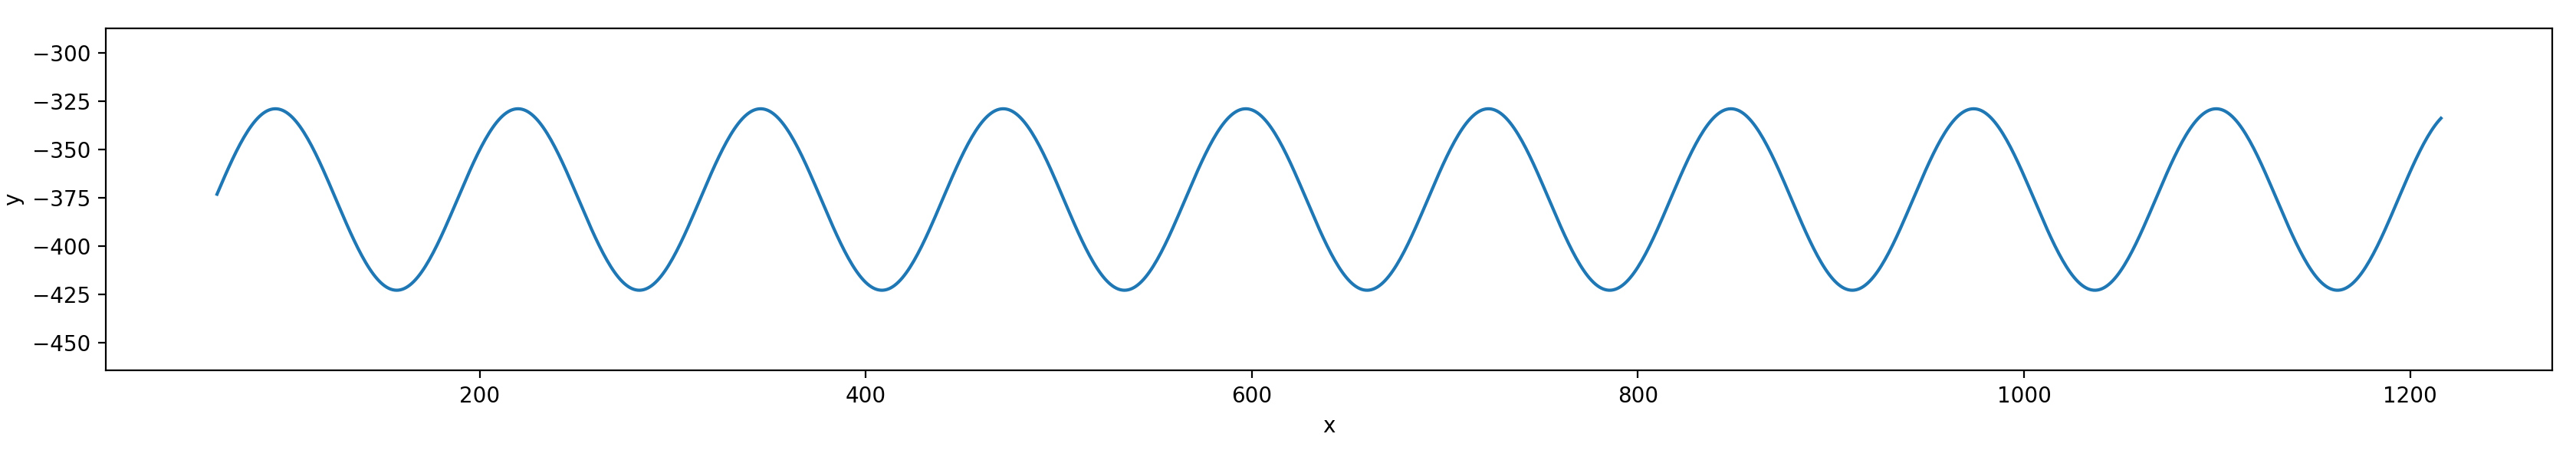
\includegraphics[width=0.85\textwidth, trim=0cm 1.5cm 0cm 0cm] {images/luria/000}
    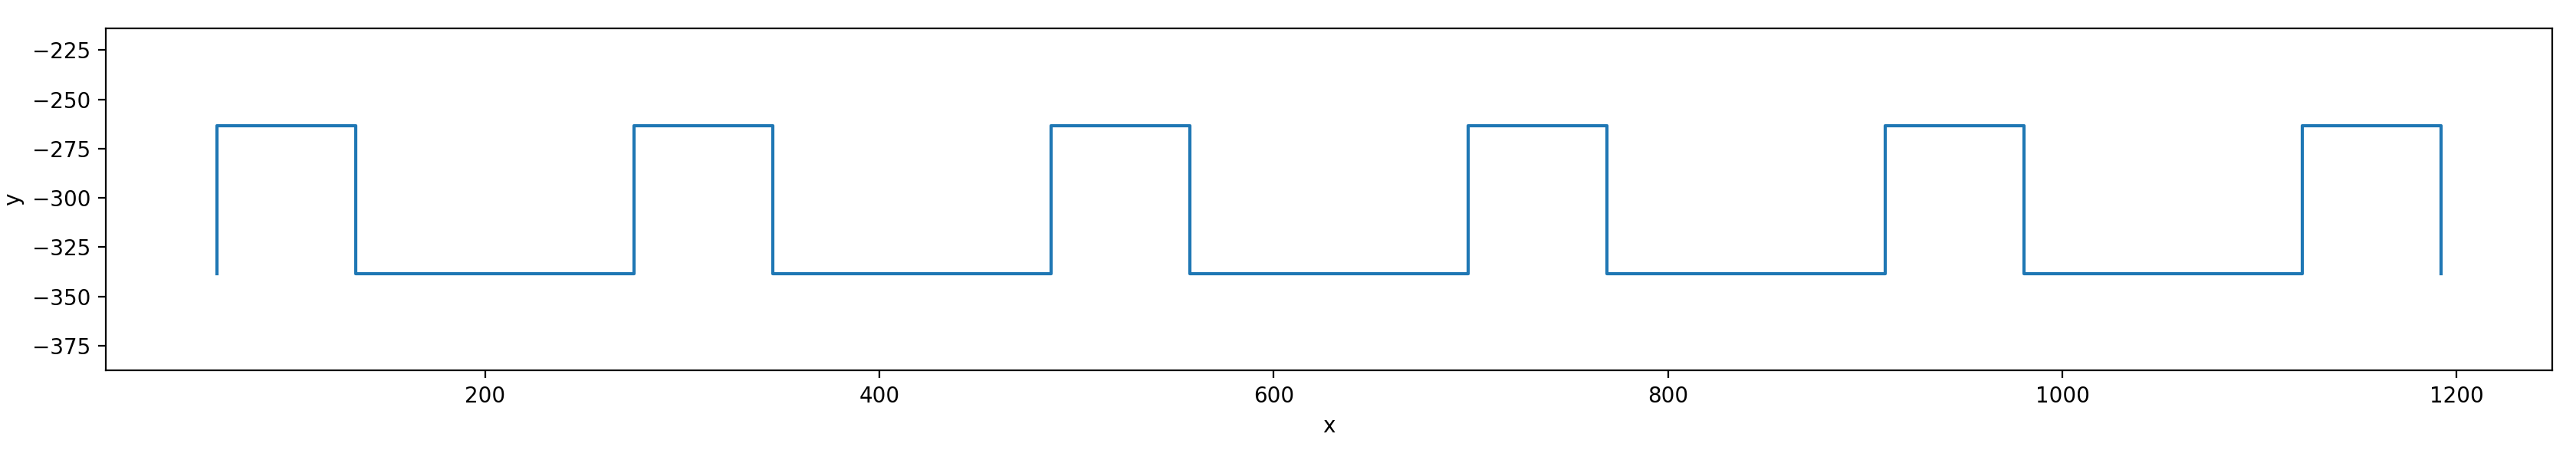
\includegraphics[width=0.85\textwidth, trim=0cm 1.5cm 0cm 0cm] {images/luria/001}
    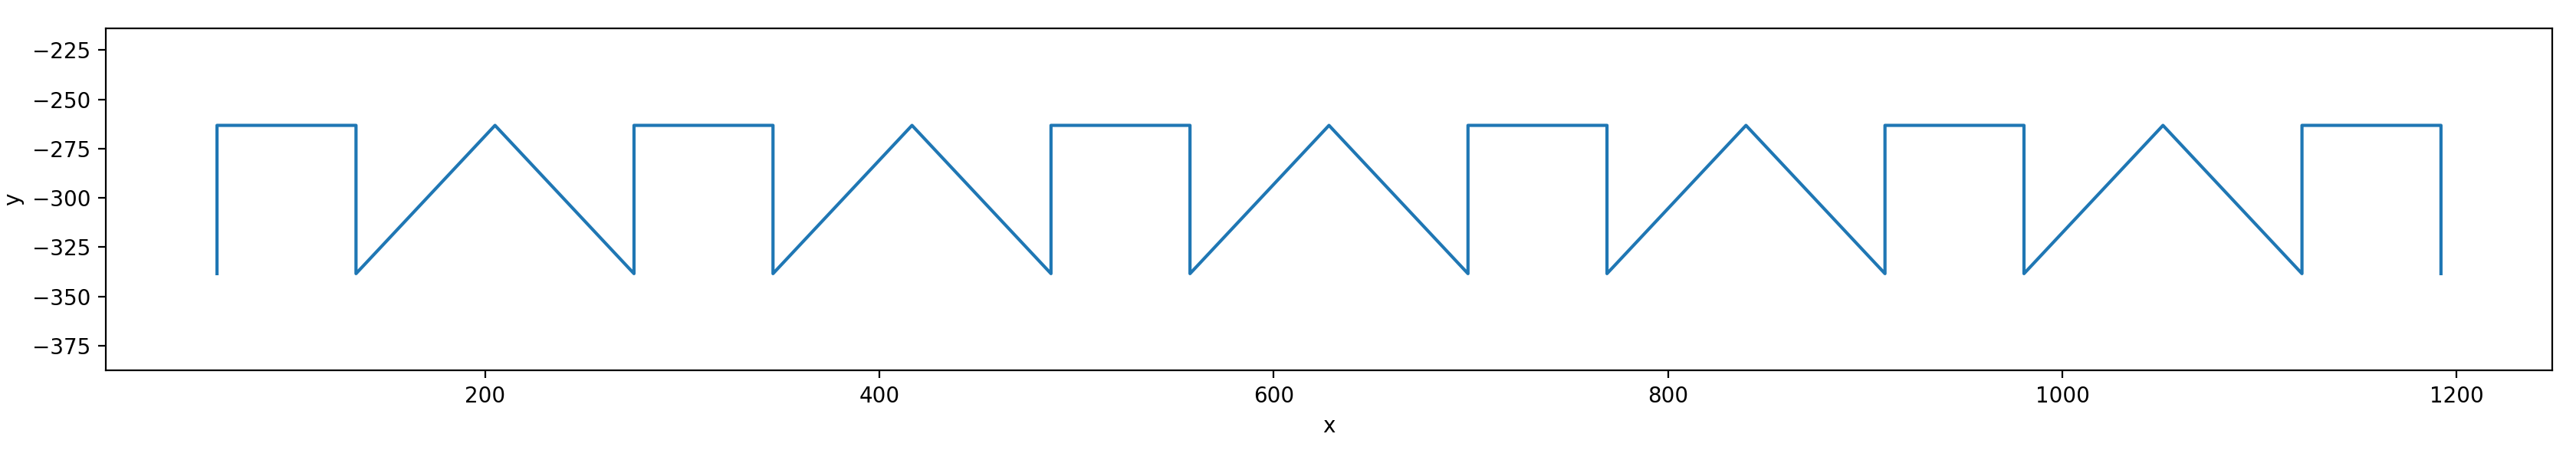
\includegraphics[width=0.85\textwidth, trim=0cm 1.5cm 0cm 0cm] {images/luria/002}
    \caption{Luria pattern types --- \textit{sinus} pattern, \textit{'P'} pattern, \textit{'PL'} pattern}
    
    \label{luria}
\end{figure}